\newpage

\chapter{Sprint 3: Breakdown Management and Intervention Planning}

\cfoot{\thepage}

\parindent=0.5in
\onehalfspacing

\section{Introduction}

Sprint 3, titled "Breakdown Management and Intervention Planning," introduces critical reactive and proactive maintenance capabilities building upon the site and equipment foundations from Sprints 1 and 2. This sprint addresses user stories US-007 (Intervention Planning), US-008 (Technician Assignment), and US-009 (Intervention Tracking) from Chapter 2's product backlog, implementing comprehensive fault reporting and scheduled maintenance management.

Network breakdowns represent urgent situations requiring immediate attention, such as power outages, equipment failures, or connectivity losses significantly impacting service quality and affecting thousands of users. The intervention planning module enables managers and engineers to schedule preventive maintenance tasks, assign technicians based on skills and availability, and track maintenance activities systematically. Together, these modules create a comprehensive maintenance management system balancing reactive problem-solving with proactive prevention strategies, directly supporting the operational requirements identified in Chapter 2 for Network Engineers and Field Technicians.

\section{Sprint Backlog}

During sprint planning, we defined the tasks required for Sprint 3 implementation. Table 5.1 presents the sprint backlog with user stories, tasks, complexity assessments, and effort estimates.

\begin{table}[H]
\centering
\small
\begin{tabular}{|p{2.5cm}|p{4cm}|p{3.2cm}|p{2.2cm}|p{1.5cm}|}
\hline
\textbf{Functionality} & \textbf{User Story} & \textbf{Tasks} & \textbf{Complexity} & \textbf{Estimate} \\
\hline

\multirow{3}{2.5cm}{Report Breakdown (US-009)} & 
\multirow{3}{4cm}{As engineer, manager, or technician, I want to report network breakdowns for quick resolution}
& Create breakdown form & Medium & 4h \\
\cline{3-5}
& & Implement severity classification & Medium & 4h \\
\cline{3-5}
& & Auto-capture downtime start & Easy & 3h \\
\hline

\multirow{3}{2.5cm}{Assign Breakdown} & 
\multirow{3}{4cm}{As manager, I want to assign breakdowns to technicians for resolution}
& Implement assignment logic & Medium & 4h \\
\cline{3-5}
& & Send notifications & Easy & 3h \\
\cline{3-5}
& & Update status workflow & Easy & 3h \\
\hline

\multirow{3}{2.5cm}{Track Resolution} & 
\multirow{3}{4cm}{As technician, I want to update breakdown status and track progress}
& Create status update interface & Easy & 3h \\
\cline{3-5}
& & Implement workflow transitions & Medium & 4h \\
\cline{3-5}
& & Capture completion data & Easy & 2h \\
\hline

\multirow{3}{2.5cm}{Monitor Impact} & 
\multirow{3}{4cm}{As manager, I want to see breakdown impact metrics and downtime}
& Display impacted users & Easy & 3h \\
\cline{3-5}
& & Calculate downtime duration & Medium & 3h \\
\cline{3-5}
& & Show impact statistics & Easy & 2h \\
\hline

\multirow{3}{2.5cm}{Schedule Intervention (US-007)} & 
\multirow{3}{4cm}{As engineer or manager, I want to schedule maintenance interventions}
& Create intervention form & Medium & 4h \\
\cline{3-5}
& & Check availability & Hard & 5h \\
\cline{3-5}
& & Prevent scheduling conflicts & Hard & 6h \\
\hline

\multirow{3}{2.5cm}{Assign Technician (US-008)} & 
\multirow{3}{4cm}{As manager, I want to assign technicians to interventions}
& Implement assignment interface & Medium & 3h \\
\cline{3-5}
& & Check workload distribution & Medium & 3h \\
\cline{3-5}
& & Send notifications & Easy & 2h \\
\hline

\multirow{3}{2.5cm}{Update Status (US-009)} & 
\multirow{3}{4cm}{As technician, I want to update intervention progress and completion}
& Create status interface & Easy & 2h \\
\cline{3-5}
& & Implement workflow & Easy & 2h \\
\cline{3-5}
& & Capture completion details & Easy & 2h \\
\hline

\multirow{3}{2.5cm}{View History} & 
\multirow{3}{4cm}{As manager, I want to view maintenance history and analytics}
& Create history view & Medium & 3h \\
\cline{3-5}
& & Filter by criteria & Medium & 3h \\
\cline{3-5}
& & Display statistics & Easy & 2h \\
\hline

\end{tabular}
\caption{Sprint 3 Backlog with Task Breakdown}
\label{tab:sprint3_backlog}
\end{table}

The backlog totals 46 hours across eight major functionalities. Conflict detection complexity stems from time overlap calculation requirements across multiple concurrent interventions. Severity-based escalation requires real-time notification infrastructure ensuring critical breakdowns receive immediate management attention.

\section{Conceptual Design}

This section presents the conceptual design models guiding Sprint 3 implementation.

\subsection{Class Diagram}

Figure 5.1 presents the class diagram introducing two core entities: Breakdown and Intervention, working with existing entities for comprehensive maintenance management.

\begin{figure}[H]
    \centering
    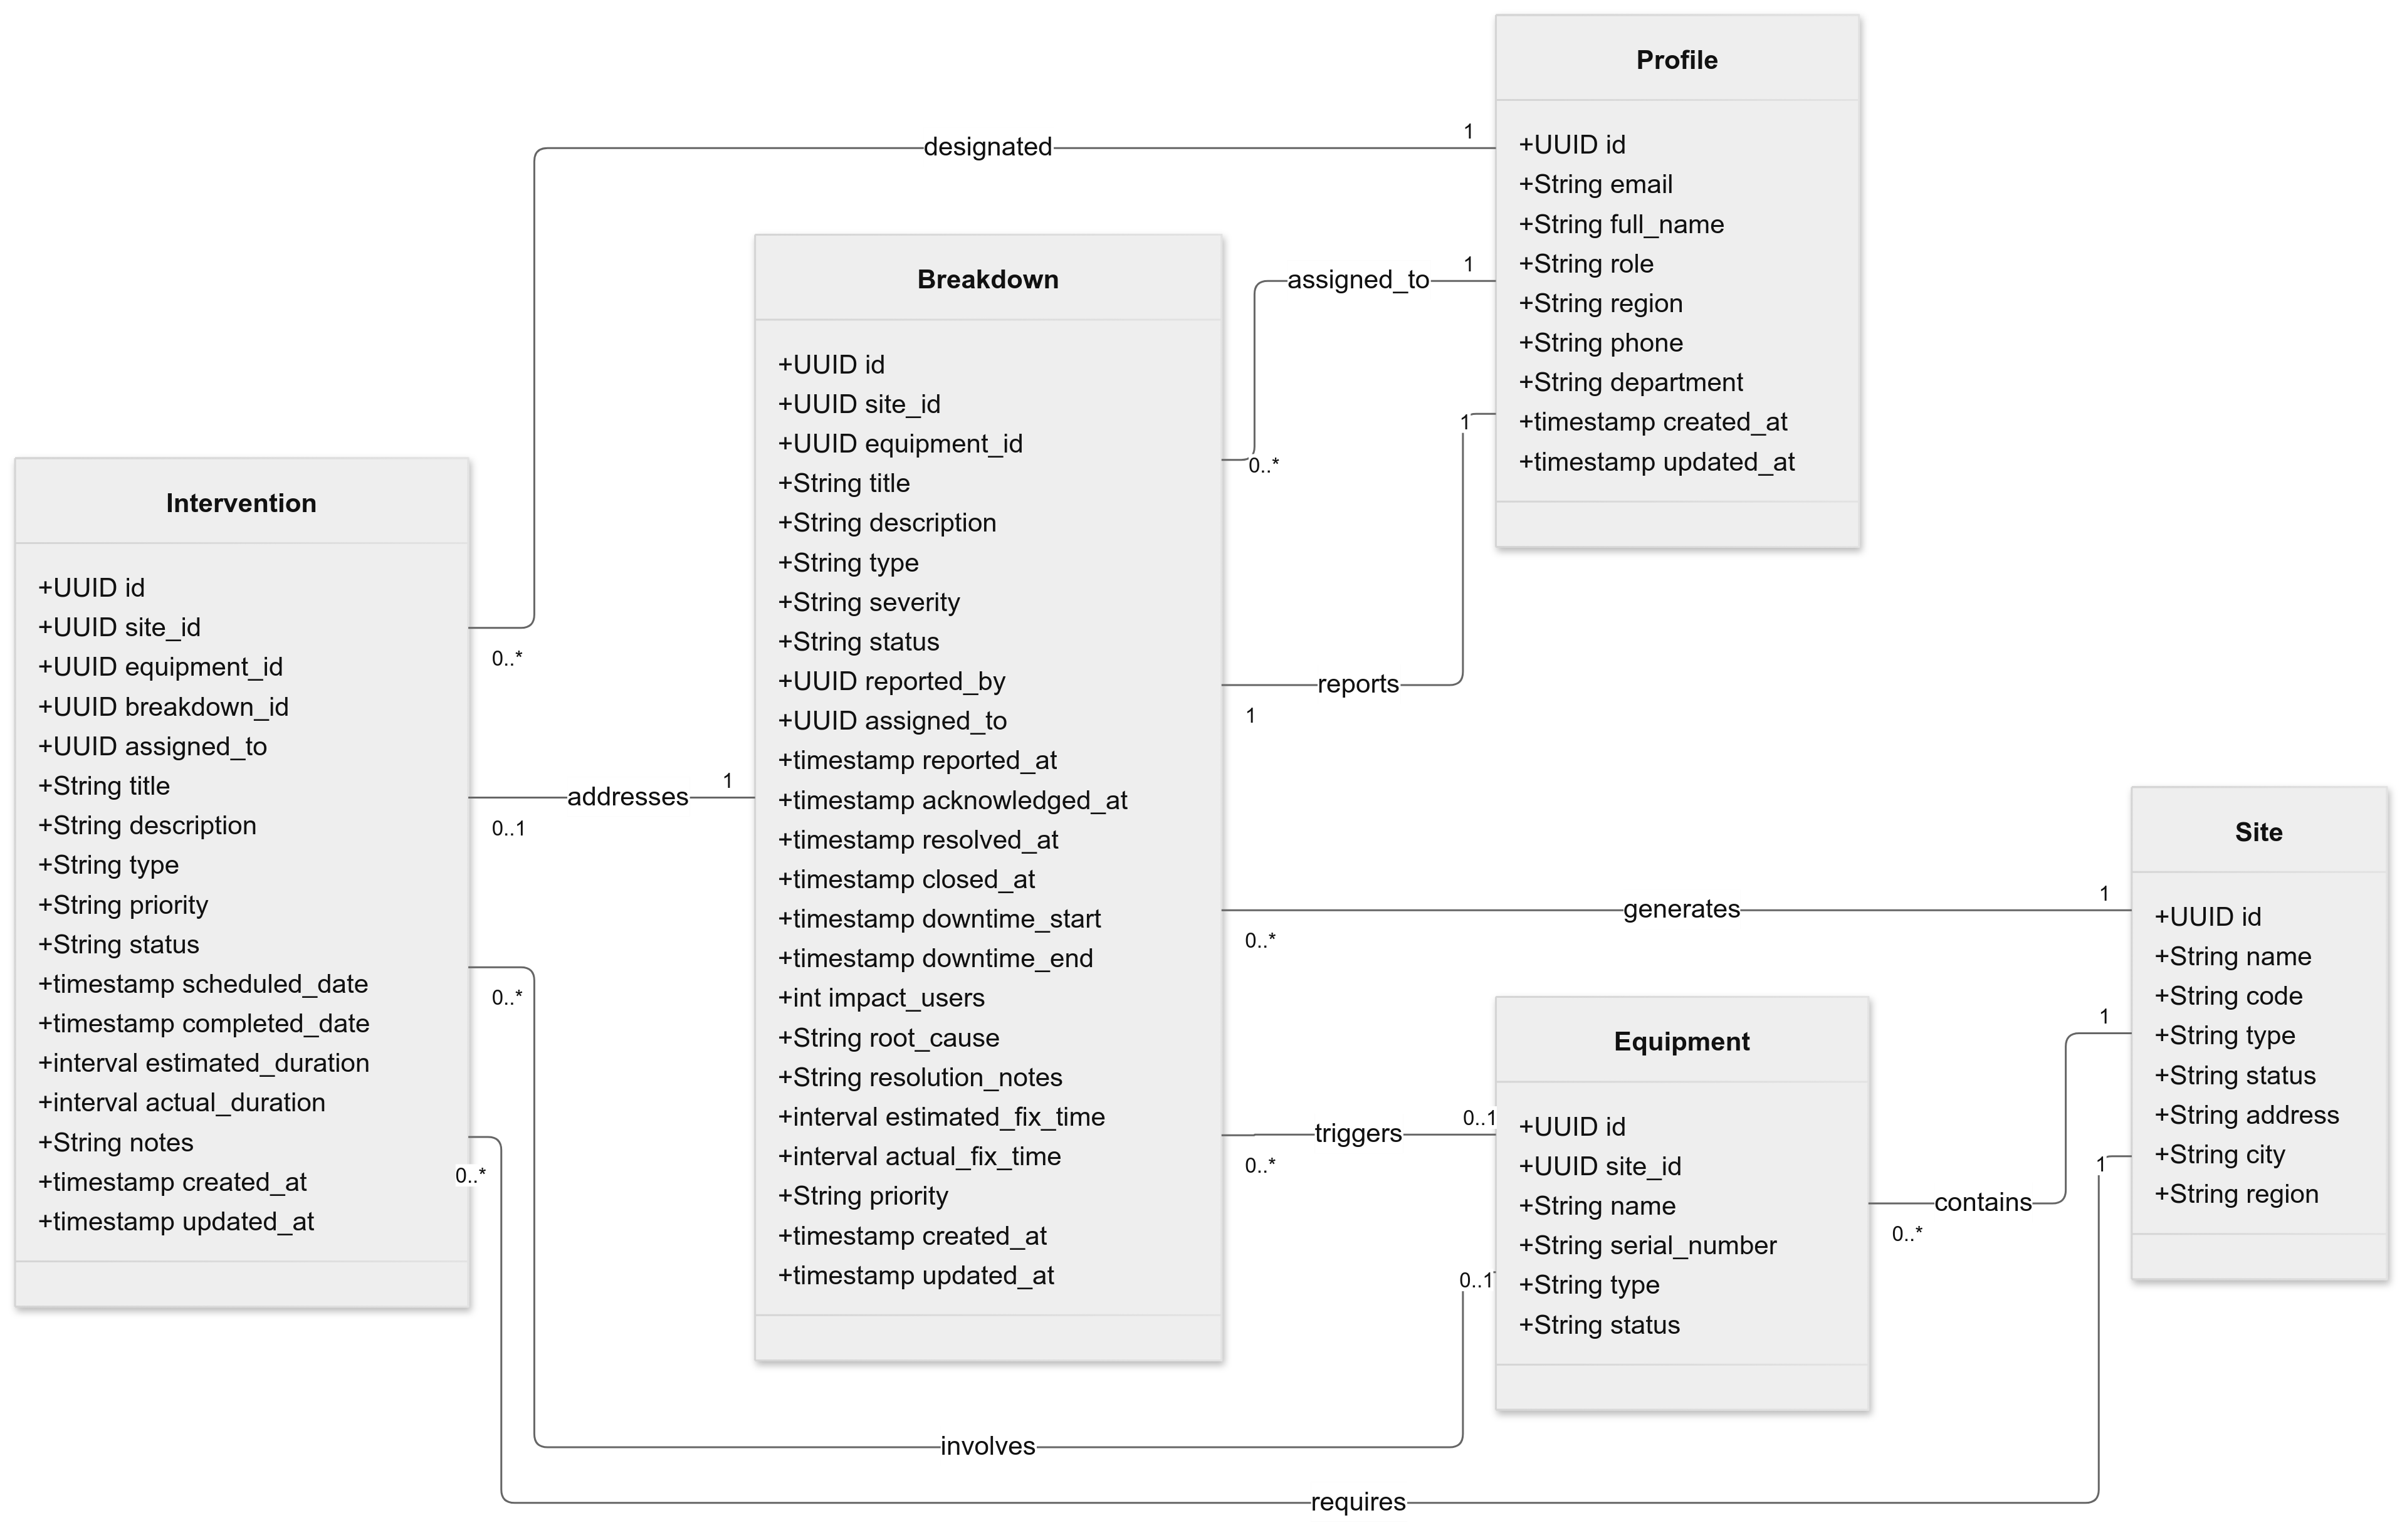
\includegraphics[width=0.95\linewidth]{img/chap_05/sprint3_class_diagram.png}
    \caption{Class Diagram - Breakdown and Intervention Management}
    \label{fig:class_diagram_sprint3}
\end{figure}


The class diagram (Figure 5.1) illustrates two primary entities using UML standard notation (name : type format). The Breakdown class represents network failures requiring immediate attention, tracking breakdown type classifications (power, hardware, software, environmental), severity levels (minor, major, critical) determining escalation procedures, and status workflow (open, investigating, in progress, resolved, closed). It maintains comprehensive timestamps capturing the entire lifecycle from initial report through resolution, tracks user impact through \texttt{impact\_users} quantifying affected subscribers, calculates downtime duration automatically from start and end timestamps, and associates with sites and equipment for geographical and asset tracking. The Intervention class manages scheduled maintenance activities, categorizing by intervention type (preventive, corrective, installation, replacement) reflecting maintenance strategy, priority levels (low, medium, high, critical) enabling resource allocation, and status tracking (scheduled, in progress, completed, cancelled). Both entities maintain associations with Profile entities for assignment tracking, Site entities for location management, and Equipment entities for asset-specific maintenance, ensuring comprehensive integration with network infrastructure established in previous sprints.

\subsection{Use Case Diagram}

Figure 5.2 presents the use case diagram employing inheritance-based permission hierarchy where each role inherits capabilities from lower roles while adding specific functionalities.

\begin{figure}[H]
    \centering
    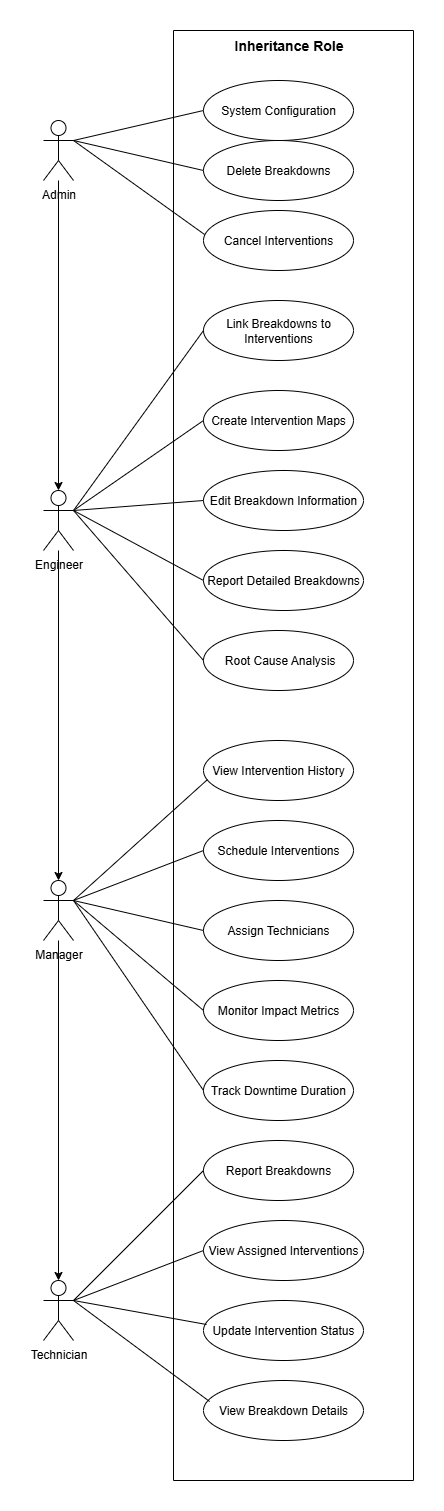
\includegraphics[width=0.3\linewidth]{img/chap_05/sprint3_usecase_diagram.png}
    \caption{Use Case Diagram - Sprint 3 with Role Inheritance}
    \label{fig:use_case_diagram_sprint3}
\end{figure}

The use case diagram (Figure 5.2) demonstrates the role inheritance hierarchy established in previous sprints. Field Technicians possess base operational capabilities including viewing assigned interventions enabling focused task management, updating intervention status providing real-time progress tracking, reporting breakdowns enabling rapid incident documentation, and viewing breakdown details supporting problem resolution. Managers inherit all technician capabilities while adding supervisory functions including viewing intervention and breakdown statistics for operational oversight, scheduling interventions enabling preventive maintenance planning, assigning technicians to interventions optimizing resource allocation, tracking downtime duration quantifying service impact, and monitoring impact metrics supporting strategic decisions. Network Engineers inherit all manager capabilities while adding technical analysis functions including conducting root cause analysis preventing recurrence, creating detailed intervention plans specifying technical procedures, editing breakdown information ensuring accurate documentation, and linking breakdowns to specific equipment supporting asset management. Administrators inherit all engineer capabilities while possessing exclusive system management rights including deleting breakdowns and interventions for data lifecycle management, cancelling scheduled interventions supporting operational flexibility, and configuring system parameters ensuring proper operation.

\textbf{Use Case Description: Report Breakdown}

Since breakdown and intervention operations share workflow patterns, we provide detailed information on the "Report Breakdown" use case as representative of Sprint 3 functionality. Table 5.2 presents the detailed textual description.

\begin{table}[H]
\centering
\small
\begin{tabular}{|p{3cm}|p{8.5cm}|}
\hline
\textbf{Element} & \textbf{Description} \\
\hline
\textbf{Use Case Name} & Report Breakdown \\
\hline
\textbf{Primary Actors} & Network Engineer, Operations Manager, Field Technician \\
\hline
\textbf{Description} & Allows users to report network breakdowns and failures requiring immediate attention with comprehensive details enabling quick resolution \\
\hline
\textbf{Pre-condition} & User authenticated with engineer, manager, or technician role; Active sites exist in system; Breakdown types configured in system \\
\hline
\textbf{Post-condition} & Breakdown record created in database; Automatic downtime tracking initiated; Notifications sent to relevant stakeholders; Critical alerts escalated to management \\
\hline
\textbf{Main Scenario} & 
1. User clicks "Report Breakdown" button
2. System displays breakdown reporting form
3. User enters breakdown title and detailed description
4. User selects breakdown type and severity level
5. User selects affected site from dropdown
6. User selects affected equipment (optional)
7. User estimates impacted users and expected resolution time
8. User submits form
9. System validates all required fields
10. System creates breakdown with auto-captured timestamp
11. System initiates downtime tracking
12. System displays success confirmation
\\
\hline
\textbf{Alternative Flows} & 
A1 - Critical Severity: At step 4, if severity selected as "Critical", system immediately notifies all managers and highlights breakdown with urgent indicator
A2 - Equipment Selection: At step 5, system dynamically loads equipment list for selected site
A3 - Auto-assignment: At step 12, system automatically assigns breakdown to available technician based on workload
\\
\hline
\textbf{Exception Scenarios} & 
E1: Missing required fields → Display field-specific error messages and return to form
E2: Invalid data entered → Display validation error with correction guidance
E3: No available sites → Display error message and disable form submission
E4: Server connection failure → Display connection error with retry option
\\
\hline
\end{tabular}
\caption{Detailed Use Case Description - Report Breakdown}
\label{tab:report_breakdown_usecase}
\end{table}

\section{Sequence Diagrams}

This section presents sequence diagrams detailing the main processes implemented in Sprint 3.

\subsection{Schedule Intervention Process}

Figure 5.3 demonstrates the complete workflow for scheduling maintenance interventions with conflict detection and technician assignment.

\begin{figure}[H]
    \centering
    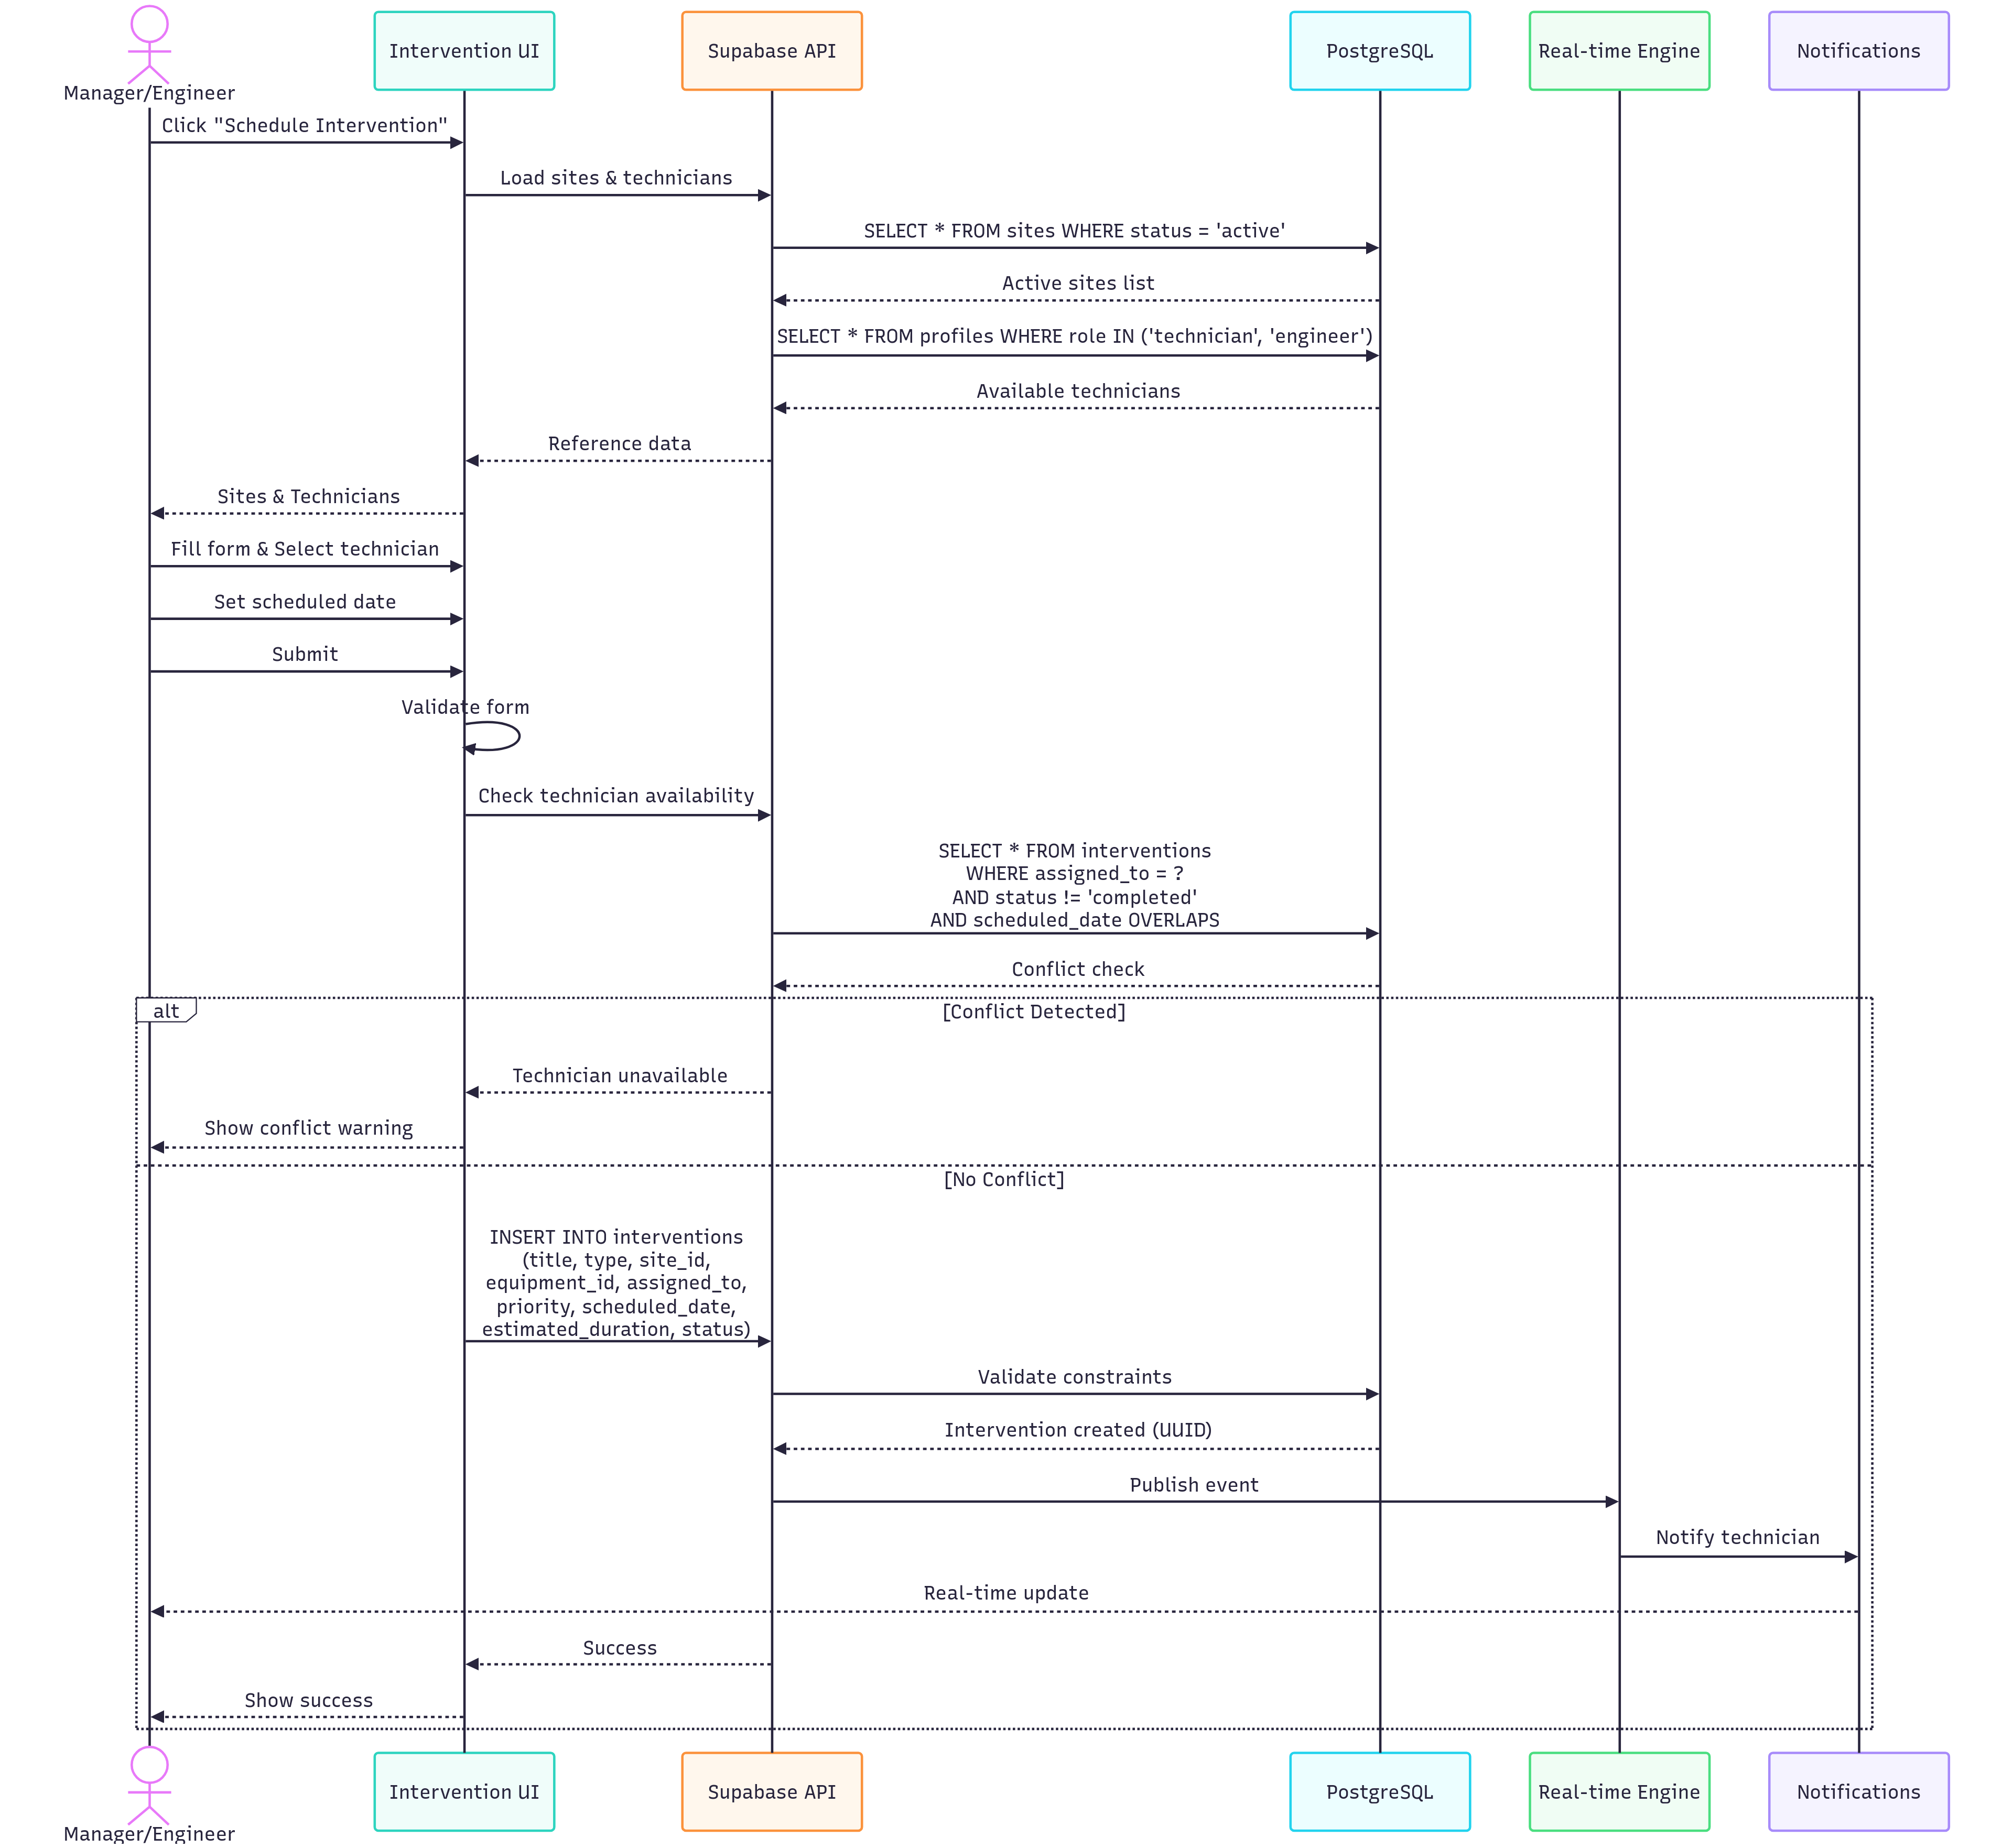
\includegraphics[width=0.95\linewidth]{img/chap_05/sprint3_sequence_intervention.png}
    \caption{Sequence Diagram - Schedule Intervention Process}
    \label{fig:sequence_schedule_intervention}
\end{figure}

\textbf{Note on Sequence Diagram:} Following UML sequence diagram standards, return messages should use dashed arrows (-->) while request messages use solid arrows (->), clearly distinguishing between calls and responses.

The schedule intervention sequence (Figure 5.3) demonstrates the workflow for planning preventive or corrective maintenance activities. An authorized user (Manager, Engineer, or Administrator) accesses the intervention management interface and clicks "Schedule Intervention" displaying the scheduling form. The user completes intervention details including descriptive title, intervention type selection (preventive, corrective, installation, replacement), priority level assignment, target site selection, optional equipment specification, technician assignment from available personnel, scheduled date and time selection, and estimated duration specification. Upon form submission, the validation system performs comprehensive checks on required fields ensuring data completeness. If validation succeeds, the system queries existing interventions for the assigned technician checking for time conflicts. The conflict detection algorithm calculates intervention time windows by adding estimated duration to scheduled start time, compares against existing commitments, and identifies overlaps. If no conflicts exist, the request proceeds to Supabase via \texttt{supabase.from('interventions').insert()} with Row Level Security verification ensuring only managers, engineers, and administrators can schedule interventions. The database creates the intervention record with "scheduled" status and sends notifications to assigned technician. The intervention list updates in real-time across all user sessions via Supabase subscriptions. If conflicts are detected, the system displays conflict details with overlapping intervention information enabling rescheduling decisions. Validation failures display specific error messages guiding correction.

\subsection{Report Breakdown Process}

Figure 5.4 illustrates the workflow for reporting network breakdowns including severity-based escalation for critical issues.

\begin{figure}[H]
    \centering
    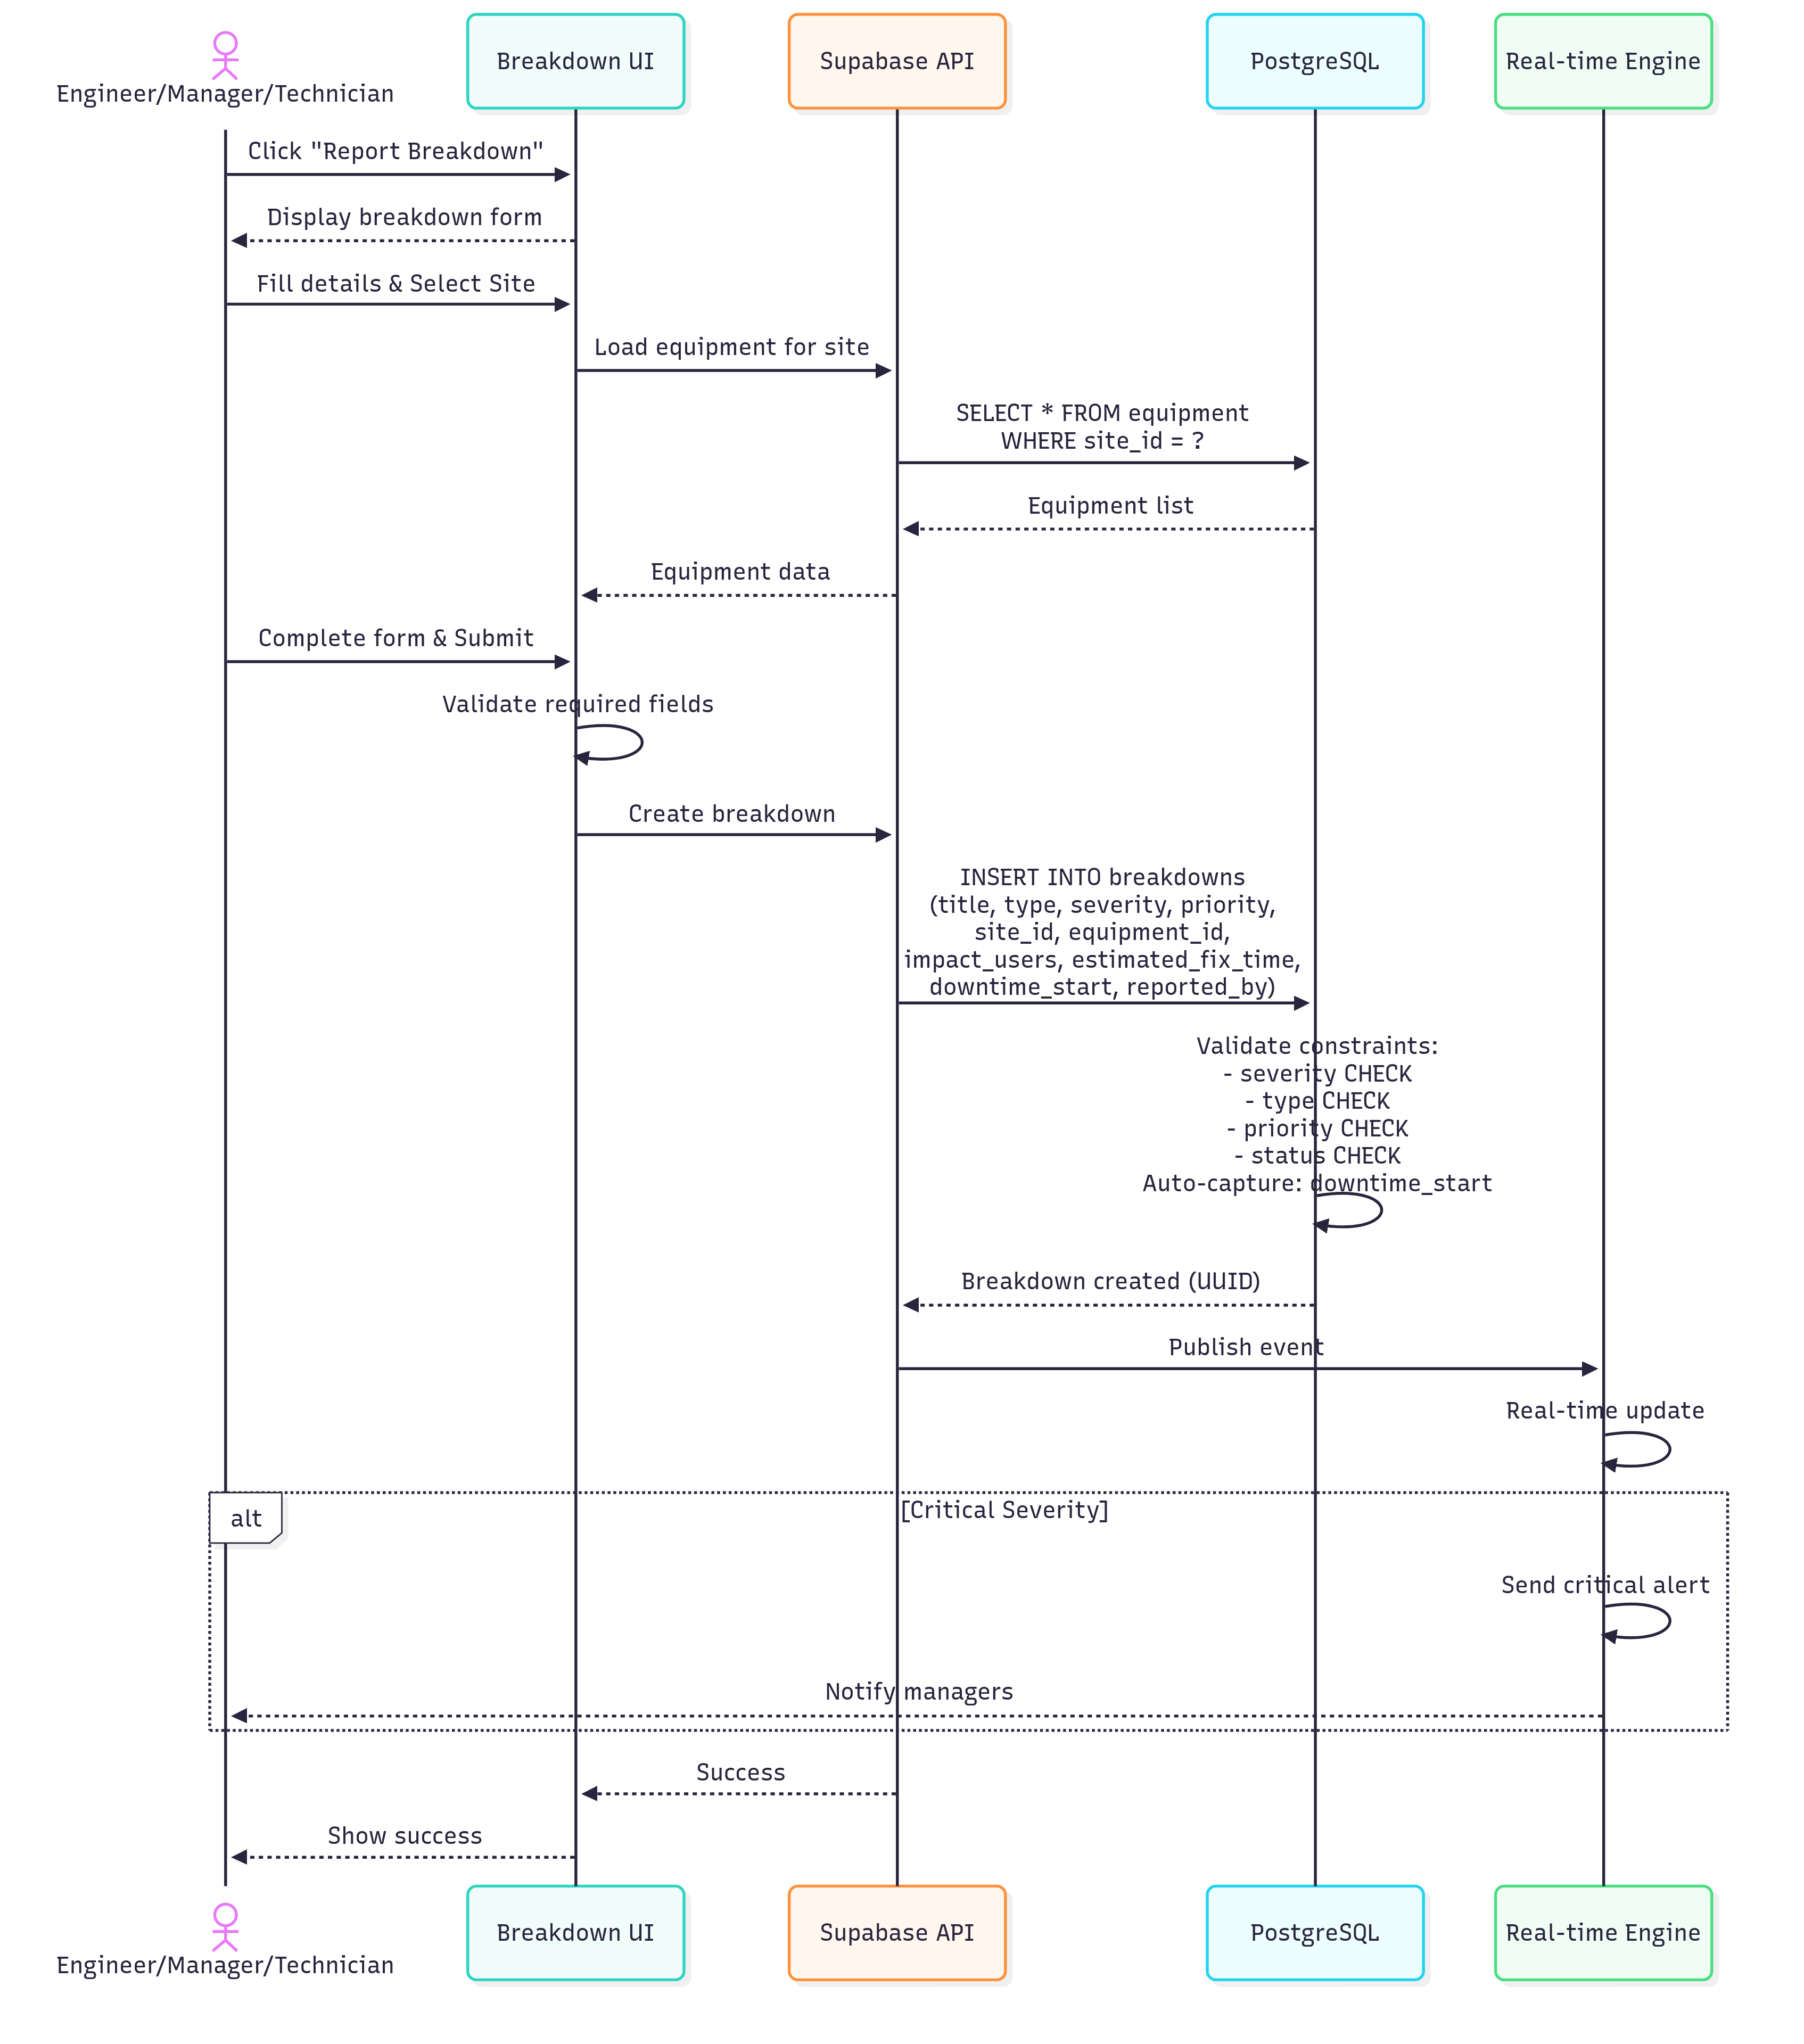
\includegraphics[width=0.95\linewidth]{img/chap_05/sprint3_sequence_breakdown.png}
    \caption{Sequence Diagram - Report Breakdown Process}
    \label{fig:sequence_report_breakdown}
\end{figure}

The report breakdown sequence (Figure 5.4) illustrates the incident reporting workflow supporting rapid response to network failures. When a user (Engineer, Manager, or Technician) identifies a network issue, they access the breakdown management interface and click "Report Breakdown" displaying the reporting form. The user provides comprehensive breakdown information including descriptive title summarizing the issue, detailed description explaining symptoms and observations, breakdown type classification (power failure, hardware malfunction, software error, environmental issue), severity level selection (minor, major, critical) determining response urgency, affected site selection from dropdown, optional affected equipment specification for asset-specific issues, and impact estimation including affected user count and expected resolution timeframe. Upon form submission, client-side validation ensures required fields are completed. Valid submissions proceed to Supabase with automatic timestamp capture recording the exact breakdown occurrence time and initiating downtime tracking. The database verifies user permissions through Row Level Security (all authenticated users can report breakdowns supporting rapid incident response) and creates the breakdown record with "open" status. If severity is marked "critical", the system immediately triggers escalation workflow sending real-time notifications to all managers and operations supervisors, displaying breakdown with urgent visual indicators, and prioritizing in management dashboards. Upon successful creation, the breakdown list updates in real-time across active sessions, the form closes, and success confirmation displays. For non-critical breakdowns, standard notification procedures apply. Validation failures display specific field errors enabling quick correction and resubmission.

\section{Implementation}

This section presents screenshots illustrating the interfaces developed during Sprint 3 implementation.

\subsection{Intervention Management Dashboard}

Figure 5.5 illustrates the intervention management dashboard providing comprehensive overview of scheduled and active maintenance activities.

\begin{figure}[H]
    \centering
    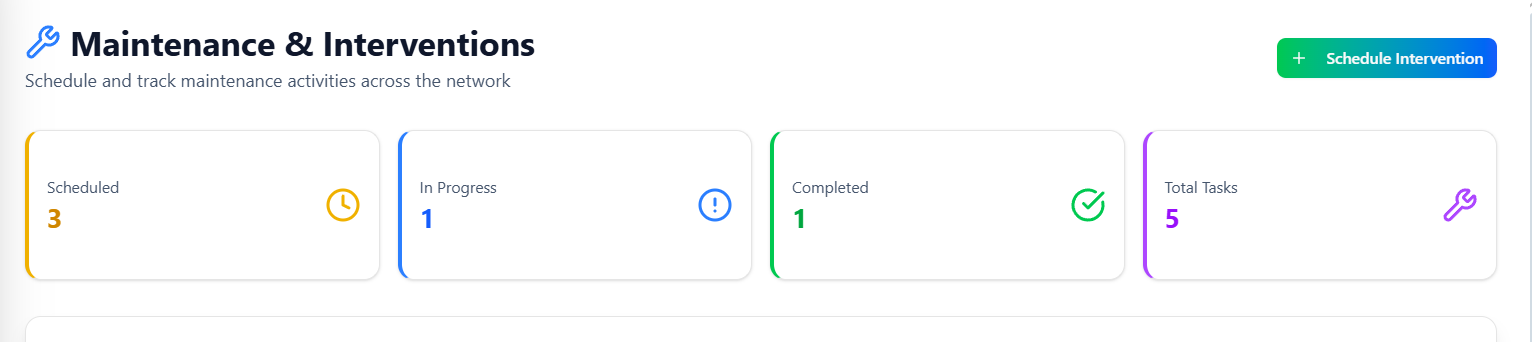
\includegraphics[width=0.9\linewidth]{img/chap_05/screenshot_interventions_dashboard.png}
    \caption{Intervention Management Dashboard with Statistics}
    \label{fig:interventions_dashboard}
\end{figure}

The intervention dashboard (Figure 5.5) displays quick statistics showing scheduled interventions awaiting execution, in-progress interventions currently being performed, and completed interventions providing historical context. The interventions table presents comprehensive task information with columns for intervention type displayed as color-coded badge, priority level with visual indicators, current status with workflow state, associated site location, assigned technician name, scheduled date and time, and action buttons (view details, update status, edit) with role-based visibility. The interface supports sorting and filtering enabling efficient task management.

\subsection{Breakdown Management Dashboard}

Figure 5.6 illustrates the breakdown management dashboard tracking network failures and their resolution status.

\begin{figure}[H]
    \centering
    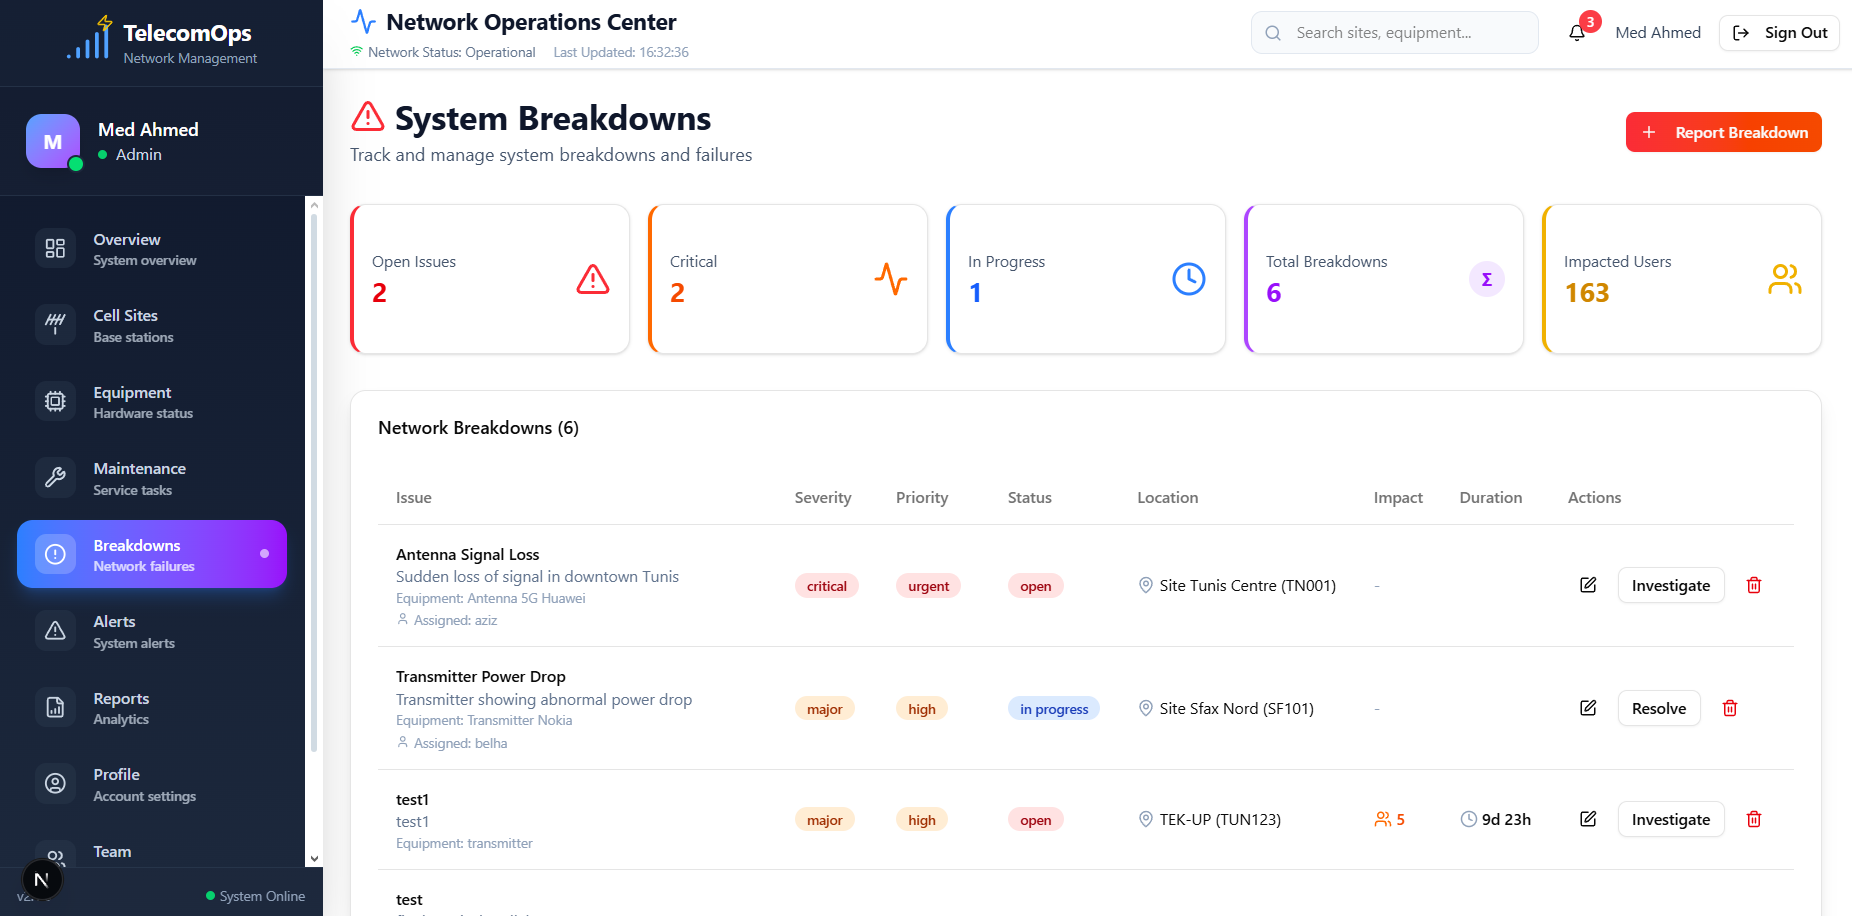
\includegraphics[width=0.9\linewidth]{img/chap_05/screenshot_breakdowns_dashboard.png}
    \caption{Breakdown Management Dashboard with Impact Metrics}
    \label{fig:breakdowns_dashboard}
\end{figure}

The breakdown dashboard (Figure 5.6) features comprehensive metrics including open issues requiring attention, critical breakdowns needing immediate response, in-progress resolutions currently being addressed, total breakdown count providing historical context, and total impacted users quantifying service impact. The breakdown table displays breakdown title with brief description, severity level with color coding (red for critical, orange for major, yellow for minor), priority assignment, current status in resolution workflow, affected site location, estimated user impact, downtime duration calculated in real-time, and action buttons (view details, assign technician, update status, resolve) with role-appropriate visibility.

\subsection{Schedule Intervention Form}

Figure 5.7 presents the intervention scheduling form enabling preventive and corrective maintenance planning.

\begin{figure}[H]
    \centering
    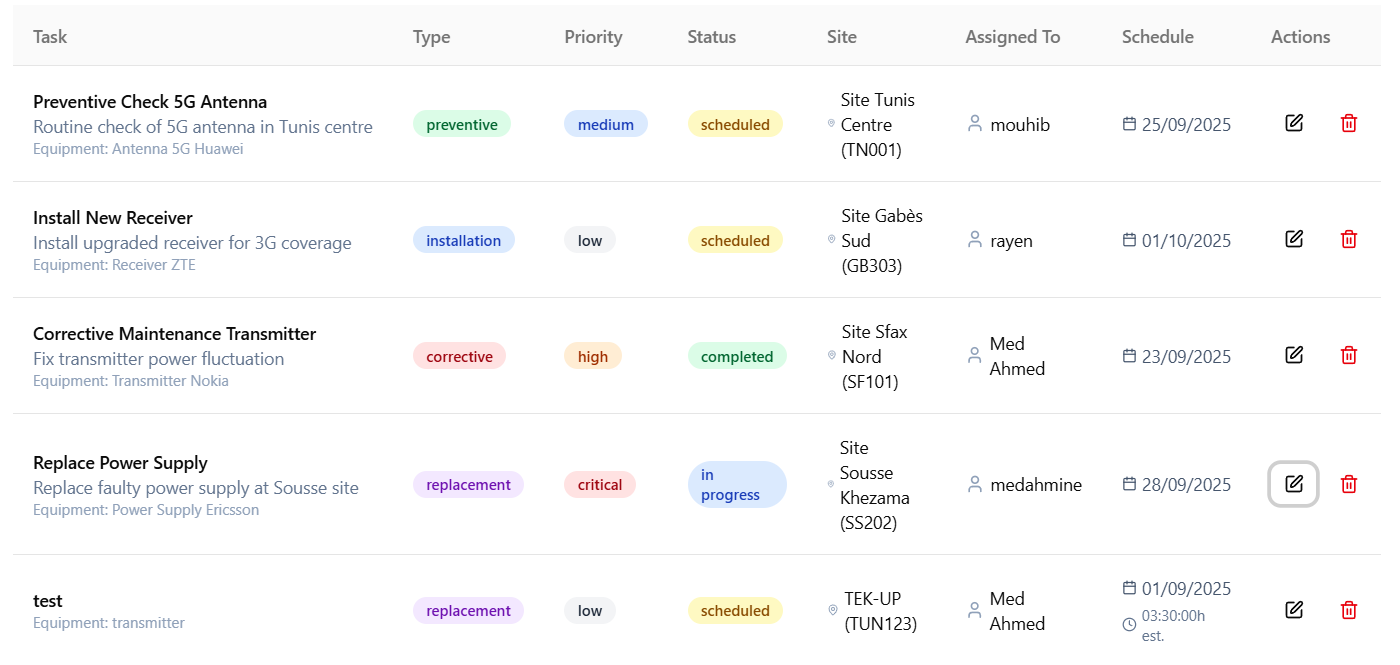
\includegraphics[width=0.7\linewidth]{img/chap_05/screenshot_schedule_intervention.png}
    \caption{Schedule Intervention Form with Conflict Detection}
    \label{fig:schedule_intervention_form}
\end{figure}

The intervention scheduling form (Figure 5.7) includes required fields for task title describing the maintenance activity, intervention type selection (preventive, corrective, installation, replacement), priority level assignment, target site dropdown with search capability, optional equipment selection for asset-specific maintenance, technician assignment from available personnel list, scheduled date picker with calendar interface, and estimated duration slider for time allocation. The form implements comprehensive validation ensuring data completeness, conflict detection alerting when technician already has scheduled interventions during proposed time, and real-time availability checking displaying technician workload. Submit action creates intervention and sends notification to assigned technician.

\subsection{Report Breakdown Form}

Figure 5.8 illustrates the breakdown reporting form enabling rapid incident documentation with severity classification.

\begin{figure}[H]
    \centering
    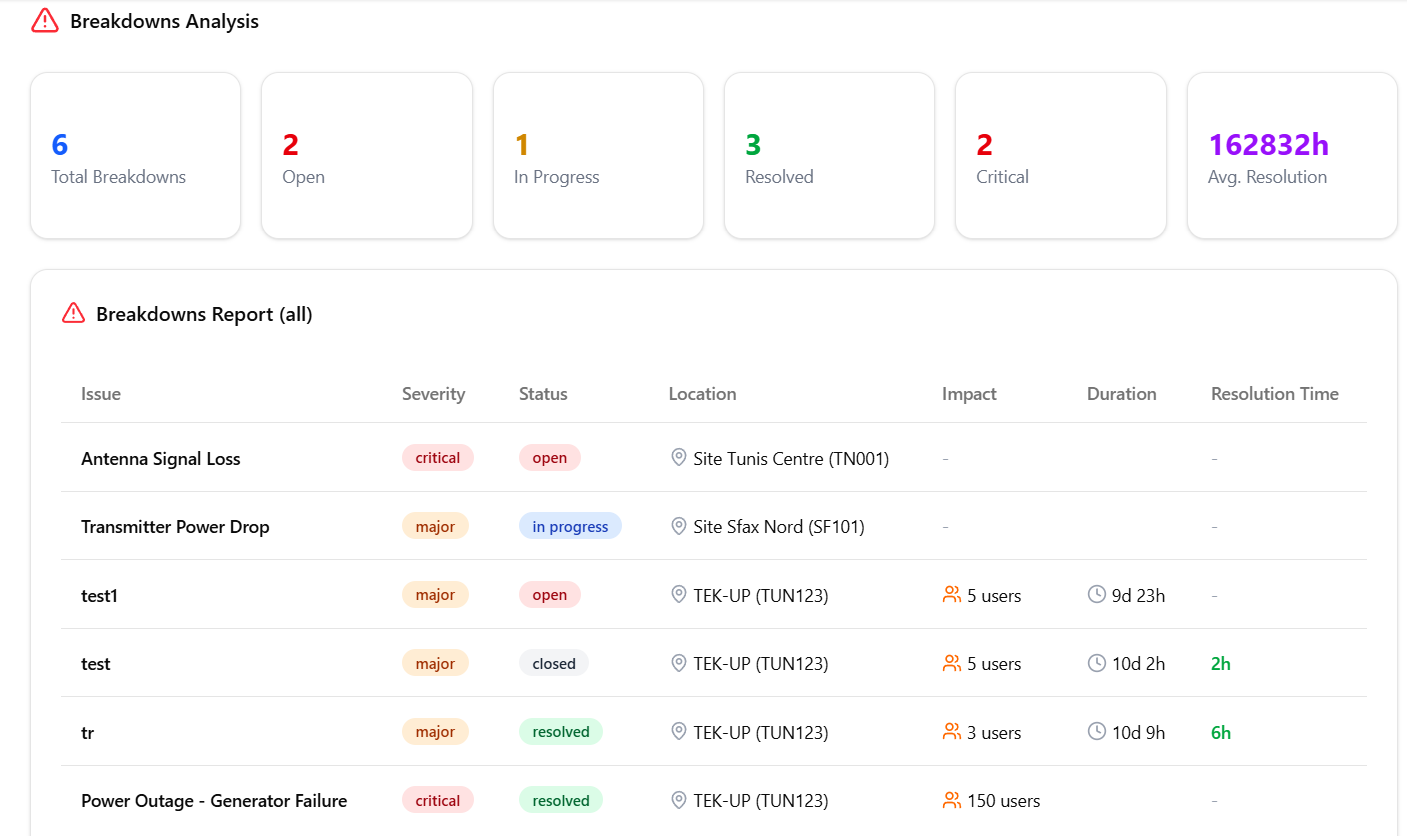
\includegraphics[width=0.7\linewidth]{img/chap_05/screenshot_report_breakdown.png}
    \caption{Report Breakdown Form with Impact Estimation}
    \label{fig:report_breakdown_form}
\end{figure}

The breakdown reporting form (Figure 5.8) enables efficient incident documentation with fields for breakdown title providing concise issue summary, detailed description explaining symptoms and context, breakdown type dropdown (power, hardware, software, environmental), severity classification (minor, major, critical) with color-coded indicators, affected site selection with search capability, optional affected equipment dropdown loading dynamically based on site selection, impact estimation including affected user count slider and expected resolution time input, and automatic downtime tracking initialization. Critical severity selection displays warning message confirming management escalation. Form validation ensures required fields completion before submission.

\section{Technical Challenges and Solutions}

Sprint 3 implementation encountered several technical challenges requiring systematic analysis and innovative solutions.

\subsection{Technician Assignment Conflict Detection}

Preventing technician double-booking when scheduling interventions required detecting time overlaps with variable-duration tasks stored as database timestamps. The challenge involved calculating intervention time windows from start time plus duration, comparing against all existing interventions for the same technician, and identifying any overlaps in the calculated time ranges. The solution implemented a conflict detection algorithm executing database queries to retrieve all interventions for the assigned technician within a relevant timeframe. The algorithm calculates each intervention's end time by adding estimated duration to scheduled start time, compares the proposed intervention's time window (start to calculated end) against existing intervention windows, and detects overlaps when proposed start falls within existing window or proposed end falls within existing window. The system displays conflict warnings with detailed information about overlapping interventions while allowing managers flexibility to override conflicts for emergency situations, supporting both conflict prevention and operational flexibility.

\subsection{Real-time Downtime Duration Calculation}

Displaying continuously updating breakdown duration in human-readable format without constant database queries or page refreshes presented performance challenges. The solution implemented client-side calculation function computing elapsed time from stored downtime start timestamp maintained in the database. The JavaScript function retrieves current time, calculates difference from downtime start timestamp, and intelligently formats duration: under 1 hour displays as "< 1h" for brevity, under 24 hours displays as hours with decimal precision, and longer durations display as days plus hours for clarity. The UI component recalculates every minute using setInterval, providing accurate current downtime information without database load, supporting real-time operational awareness while maintaining system performance.

\subsection{Cascading Status Updates and Timestamp Management}

Multiple status transitions requiring automatic timestamp capture (acknowledged, investigating, resolved, closed) without manual entry while triggering related actions like downtime calculation and notification delivery required careful workflow design. The solution implemented automatic timestamp capture in database update logic by detecting status changes through comparison of old and new values. When breakdown status transitions to "investigating", the system automatically sets \texttt{acknowledged\_at} timestamp; when transitioning to "resolved", sets both \texttt{resolved\_at} and \texttt{downtime\_end} timestamps enabling automatic duration calculation; and when transitioning to "closed", verifies all prior timestamps exist ensuring workflow compliance. This approach ensures data consistency, provides accurate audit trails for compliance requirements, eliminates manual timestamp entry reducing user workload, and triggers appropriate notifications and dashboard updates maintaining stakeholder awareness throughout the resolution process.

\section{Testing and Validation}

Sprint 3 underwent comprehensive testing ensuring reliability, workflow integrity, and proper integration with existing system components.

\subsection{Functional Testing}

Functional testing verified all Sprint 3 features operate correctly according to specifications. Breakdown reporting tests validated form submission with all severity levels, confirmed critical breakdowns trigger immediate manager notifications through real-time channels, verified automatic downtime tracking initialization with accurate timestamp capture, and ensured proper status workflow transitions through all states (open, investigating, in progress, resolved, closed). Intervention scheduling tests validated form submission for all intervention types (preventive, corrective, installation, replacement), confirmed technician assignment with workload checking, verified conflict detection identifies overlapping time slots accurately, and ensured notification delivery to assigned technicians. Status update tests confirmed workflow transitions respect role permissions, verified automatic timestamp capture for all transition points, and ensured real-time dashboard updates reflect current system state. CRUD operations for both breakdowns and interventions ensured data integrity with proper validation and constraint enforcement.

\subsection{Integration Testing}

Integration testing ensured Sprint 3 components work seamlessly with existing modules from Sprints 1 and 2. Site and equipment integration tests verified resource selection when reporting breakdowns, confirmed equipment dropdown population based on selected site, and ensured proper foreign key relationships maintain referential integrity. Authentication and authorization tests verified role-based permission hierarchy works correctly, confirmed managers can schedule interventions while technicians can only update status, and ensured administrators possess all privileges. Real-time notification tests confirmed managers receive critical breakdown alerts immediately, verified technicians receive intervention assignment notifications, and ensured notification delivery across multiple devices and browsers. Database relationship tests verified foreign key enforcement prevents orphaned records, confirmed cascade behaviors work correctly, and ensured referential integrity maintained during record deletion. Dashboard statistics tests validated accurate calculation from source data, confirmed real-time recalculation when underlying data changes, and ensured statistics match manual counts.

\subsection{User Acceptance Testing}

Tunisia Telecom operational staff tested Sprint 3 features in realistic scenarios providing valuable feedback. Technicians tested mobile-responsive interfaces for field breakdown reporting, confirmed form usability with touch interfaces, validated intervention status updates from field locations, and appreciated automatic downtime tracking reducing manual data entry. Managers tested intervention scheduling workflows, validated conflict detection preventing scheduling errors, confirmed priority indicators help resource allocation decisions, and appreciated real-time dashboard updates enabling proactive management. Engineers tested breakdown reporting with comprehensive technical details, confirmed adequate description fields for documentation requirements, validated equipment association functionality supporting asset tracking, and appreciated proper status transition workflows guiding resolution process. Overall feedback was positive with users appreciating clear visual indicators for severity and priority, intuitive workflows requiring minimal training, real-time updates providing current operational awareness, and mobile optimization supporting field operations. Minor improvement suggestions were noted for future enhancement consideration.

\subsection{Performance Testing}

Performance validation confirmed Sprint 3 meets NFR-001 requirements from Chapter 2. Dashboard load times averaged 1.8 seconds with 100+ active breakdowns and interventions, conflict detection queries execute within 150ms even with 500+ scheduled interventions per technician, real-time notification delivery averages 1.2 seconds from event occurrence to user notification, and downtime duration calculations execute client-side with negligible performance impact. All performance metrics exceed established targets ensuring responsive user experience under operational load.

\section{Sprint Review and Retrospective}

Sprint 3 review with stakeholders confirmed successful delivery of all committed user stories addressing US-007, US-008, and US-009. Stakeholders particularly valued the severity-based escalation ensuring critical issues receive immediate attention, conflict detection preventing technician scheduling errors and resource conflicts, comprehensive impact tracking quantifying service disruption for reporting, and mobile-optimized interfaces supporting field technician operations. User acceptance testing across all four user roles validated the implementation meets telecommunications maintenance management requirements.

The sprint retrospective identified positive outcomes including Supabase real-time subscriptions enabling immediate notification delivery critical for urgent breakdown response, comprehensive workflow design guiding users through proper resolution processes, TypeScript type safety preventing status transition errors during development, and excellent stakeholder engagement throughout sprint ensuring requirements alignment. Areas for improvement include earlier mobile device testing to identify touch interface optimization opportunities, more extensive performance testing with production-scale data volumes, additional user training materials for complex workflows, and enhanced documentation for troubleshooting common issues.

\section{Conclusion}

Sprint 3 successfully delivered comprehensive breakdown management and intervention planning capabilities significantly enhancing TelecomOps maintenance functionality. The implementation addressed all committed user stories (US-007, US-008, US-009) from Chapter 2's product backlog, providing complete breakdown lifecycle management from initial report through resolution and comprehensive intervention planning supporting preventive and corrective maintenance strategies.

The breakdown management system enables rapid incident reporting with detailed severity classification, automatic downtime tracking quantifying service impact, workflow-guided resolution ensuring systematic problem-solving, and critical severity escalation ensuring urgent issues receive immediate management attention minimizing customer impact. The intervention planning module enables proactive maintenance scheduling with intelligent conflict detection preventing resource double-booking, technician assignment based on availability and workload, comprehensive progress tracking providing operational visibility, and proper integration with site and equipment management supporting asset-specific maintenance.

Together, these modules create a complete maintenance solution balancing reactive breakdown response with proactive intervention planning. Integration with existing modules from Sprints 1 and 2 ensures proper site and equipment association, comprehensive asset tracking, and unified operational workflows. Role-based permissions provide appropriate access levels reflecting organizational hierarchy while real-time notifications keep stakeholders informed enabling rapid coordination and response.

Technical challenges around conflict detection, timestamp management, and real-time duration calculation were successfully resolved through careful algorithm design, automatic data capture, and client-side computation. Comprehensive testing including functional validation, integration verification, user acceptance testing, and performance validation confirmed the implementation meets all requirements and performs well under operational load.

Sprint 3 establishes foundation for advanced maintenance analytics and predictive capabilities. The comprehensive breakdown and intervention data enables pattern analysis identifying recurring issues, supports maintenance schedule optimization based on historical performance, facilitates resource allocation improvement through workload analytics, and enables predictive maintenance strategies reducing unplanned downtime. Quality metrics exceeded established targets with successful stakeholder validation and performance exceeding NFR-001 requirements.

The next chapter presents Sprint 4, titled "Alert System and Energy Consumption Monitoring," which extends operational capabilities with real-time alert generation based on equipment status and site conditions, and comprehensive energy consumption tracking supporting cost management and sustainability initiatives, addressing user stories US-010, US-011A-B from the product backlog.